\chapter{Machine learning methods}
\label{chap2}

The field of \emph{machine learning (ML)} is a complex discipline grounded in the language of probability theory, statistics, and information theory. In this chapter, we describe all the methods and ML techniques applied in the practical part of this thesis. However, these are based on a deeper understanding of ML concepts. Since this knowledge is not part of the standard curriculum of our study program, the fundamentals of ML are included in an extensive appendix of this thesis, and we will frequently refer to terms explained there.

\section{Model architecture} 
In their essence, neural networks are function approximations and in practice we leverage them to estimate the probability distribution. Given input data $\bm{x}$, a neural network learns a mapping $f_\theta(\bm{x})$ parameterized by weights $\theta$, such that $f_\theta(\bm{x})$ gives a meaningful output. The \emph{model architecture} creates the backbone for such function, and have big influence on its quality. Many different neural network architectures were proposed in the realm of computer vision. Two basic ones we want to explore are \emph{fully connected networks} and \emph{convolutional neural networks (CNNs)}. Convolutional networks, however, came through a lot of development and many succesfull image recognition architectures were established, some of which we put into test in our experiments.

\subsection{Activation functions}

One of the hyperparameters we are interested in exploring is the \emph{activation function}. Activation functions introduce non-linearity into neural networks, enabling them to approximate more complex functions. Choosing the right activation function can impact training dynamics, stability, and ultimately model performance. In this subsection, we describe the activation functions used in our work.

\paragraph{ReLU}

The \emph{Rectified Linear Unit (ReLU)} is one of the most widely used activations due to its simplicity and effective gradient propagation:

\begin{equation}
    \mathrm{ReLU}(x) = \max(0, x).
\end{equation}

\paragraph{Leaky ReLU}

By design, ReLU ignores half of the activations, which can obstruct the training. \emph{Leaky ReLU} addresses this by allowing still smaller, but non-zero gradient even for the negative activations:

\begin{equation}
    \mathrm{LeakyReLU}(x) = 
    \begin{cases}
        x, & x \ge 0, \\
        \alpha x, & x < 0,
    \end{cases}
\end{equation}

where typically $\alpha = 0.01$.

\paragraph{ELU}

The idea of \emph{Exponential Linear Unit (ELU)} is similar to the Leaky ReLU, but ELU is smooth:

\begin{equation}
    \mathrm{ELU}(x) = 
    \begin{cases}
        x, & x \ge 0, \\
        \alpha (e^x - 1), & x < 0,
    \end{cases}
\end{equation}

where $\alpha$ is a hyperparameter controlling the value to which ELU saturates for negative inputs.

\paragraph{SELU}

The \emph{Scaled Exponential Linear Unit (SELU)} is defined as:

\begin{equation}
    \mathrm{SELU}(x) = \lambda \cdot
    \begin{cases}
        x, & x \ge 0, \\
        \alpha (e^x - 1), & x < 0,
    \end{cases}
\end{equation}

with specific fixed parameters $\lambda \approx 1.0507$ and $\alpha \approx 1.6733$. SELU is designed for self-normalizing networks, maintaining mean and variance under certain conditions \cite{klambauer2017selfnormalizingneuralnetworks}.

\paragraph{GELU}

The \emph{Gaussian Error Linear Unit (GELU)} is a probabilistic gating with an empirical success in many deep learning domains \cite{hendrycks2023gaussianerrorlinearunits}:

\begin{equation}
    \mathrm{GELU}(x) = x \cdot \Phi(x),
\end{equation}

where $\Phi(x)$ is the standard normal cumulative distribution function. An approximation often used in practice is:

\begin{equation}
    \mathrm{GELU}(x) \approx 0.5\, x \left[1 + \tanh\left(\sqrt{\frac{2}{\pi}} \left(x + 0.044715\, x^3\right)\right)\right].
\end{equation}

All of the activation functions described earlier are can be used in the hidden layers of a neural network. These however, do not work well for the output layer. The two most common choices for \emph{classification heads} are the \emph{sigmoid} and \emph{softmax} functions.

\paragraph{Sigmoid}

The \emph{sigmoid} function is typically used in binary classification, to model probabilities in $[0, 1]$:

\begin{equation}
    \sigma(x) = \frac{1}{1 + e^{-x}}.
\end{equation}

\paragraph{Softmax}

\emph{Softmax} is the most common activation function for classification into multiple classes, as the output of \emph{softmax} can be directly interpreted as a probability distribution over classes:

\begin{equation}
    \mathrm{softmax}(x_i) = \frac{e^{x_i}}{\sum_j e^{x_j}}.
\end{equation}

In our experiments, we use either $3$ sigmoids (normalized afterwards to $1$), or a softmax activations as the classification heads.

\subsection{Fully connected network}

A fully connected neural network, often referred to as a \emph{dense neural network} or \emph{multilayer perceptron (MLP)}, is one of the fundamental architectures in machine learning. It consists of sequential layers where each neuron in one layer is connected to every neuron in the following layer.

The general structure is simple: the network has an \emph{input layer}, several \emph{hidden layers}, and an \emph{output layer}. Each layer transforms its input vector into an output vector through a combination of a linear transformation and a non-linear activation function.

Formally, the operation of a fully connected layer can be described as:

\begin{equation} 
	\label{eq:fully-connected} \bm{h} = \phi(\bm{W}\bm{x} + \bm{b}), 
\end{equation}

where $\bm{x}$ is the input vector, $\bm{W}$ is the weight matrix, $\bm{b}$ is the bias vector, $\phi$ is a non-linear activation function (such as ReLU or sigmoid), and $\bm{h}$ is the resulting output (also called the hidden state).

\begin{figure}[h]
  \centering
  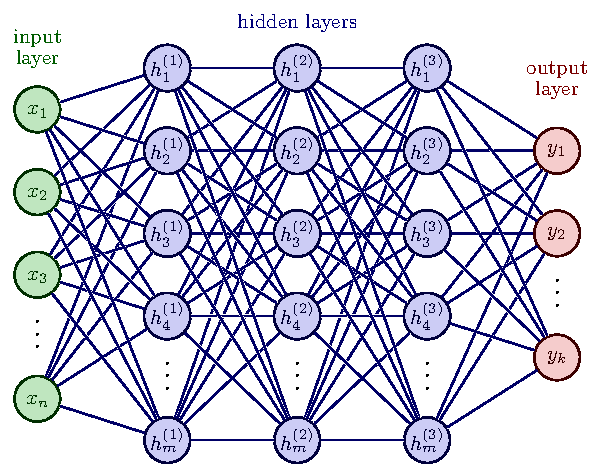
\includegraphics[width=0.9\textwidth]{img/neural_networks.pdf}
  \caption{Dense neural network \cite{neural_networks_image}.}
  \label{fig:dense_network}
\end{figure}

In the context of classification, the final output layer typically applies a softmax activation function to produce a probability distribution over the possible classes.

While fully connected networks can in principle approximate any continuous function, they tend to be inefficient for structured inputs like images. This inefficiency motivated the development of specialized architectures, such as convolutional neural networks.

\subsection{Convolutional network}

Convolutional neural networks (CNNs) \cite{bengio2017deep} are designed to process data with a grid-like structure, for example 1-D sequences or 2-D images. Unlike fully connected networks, CNNs capture the spatial structure of the data while greatly reducing the number of parameters.

\paragraph{Computation of convolution}

At the heart of a CNN is the \emph{convolutional layer}, where a small filter (also called a kernel) slides across the input and computes local dot products. Mathematically, a 2D convolution operation between an input $\bm{I}$ and a filter $\bm{K}$ can be expressed as:

\begin{equation} 
	\label{eq:convolution} 
	(\bm{I} * \bm{K})(i,j) = \sum_{m}\sum_{n} \bm{I}(i+m, j+n) , \bm{K}(m,n), 
\end{equation}

where $(i,j)$ are the spatial coordinates of the output, and the sums run over the spatial extent of the filter. The output of this operation is then refered to as \emph{feature map}.

\begin{figure}[h!]
  \centering
  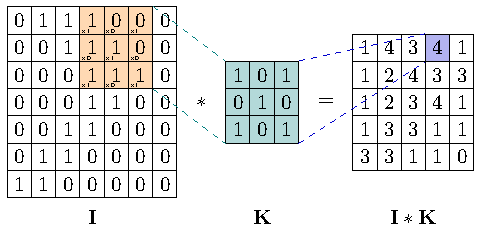
\includegraphics[width=0.9\textwidth]{img/conv2d.pdf}
  \caption{Applying single 2D convolutional kernel \cite{conv2d_image}.}
  \label{fig:conv2d}
\end{figure}

The filter does not have to slide over every input location, but can move in larger steps given by the \emph{stride}. A stride of $(s_h, s_w)$ skips $s_h$ rows and $s_w$ columns between successive applications of the filter. This effectively reduces the spatial dimension of the feature map, which can help.

\paragraph{Pooling layers}

Other way to reduce the spatial dimensions in CNNs is provided by \emph{pooling layers}. The most common variant is \emph{max pooling}, which down-samples the input by taking the maximum value over non-overlapping regions. For example, a $2\times2$ max pooling operation reduces each $2\times2$ region to a single value:

\begin{equation} 
	\label{eq:max-pooling} 
	y(i,j) = \max_{(m,n) \in \mathcal{R}(i,j)} I(m,n), 
\end{equation}

where $\mathcal{R}(i,j)$ denotes the receptive field corresponding to output location $(i,j)$. An alternative to max pooling is \emph{average pooling}, which computes the average value within each region instead of the maximum:

\begin{equation}
	\label{eq:avg-pooling}
	y(i,j) = \frac{1}{|\mathcal{R}(i,j)|} \sum_{(m,n) \in \mathcal{R}(i,j)} I(m,n),
\end{equation}


In our experiments we always use the $2\times2$ receptive fields. 

\paragraph{Depthwise separable convolutions}

Standard convolutions are computationally expensive, especially when both the input and output have many channels. One way to alleviate this is by using \emph{depthwise separable convolutions}, which decompose a convolution into two simpler operations:

\begin{itemize} 
	\item \textbf{Depthwise convolution:} A spatial convolution is applied independently to each input channel. 
	\item \textbf{Pointwise convolution:} A $1\times1$ convolution is applied across channels to mix the features. 
\end{itemize}

This decomposition significantly reduces computational cost and the number of parameters, while often maintaining or  improving performance.

\paragraph{Transition to fully connected layer}

After several stages of convolutions and pooling we end up with the high-level feature maps. We must convert these into a form suitable for classification. This is typically achieved by flattening the feature maps into a 1D vector and feeding it into one or more fully connected layers. These final layers map the learned feature representations to the output classes.

Another popular way to transition from convolutional feature maps to dense layers is \emph{global average pooling (GAP)}. Instead of flattening the entire feature map, which can result in a large number of parameters and lead to overfitting, GAP computes the average of each feature map individually. This results in a single scalar value per feature map, significantly reducing the dimensionality while preserving spatially aggregated information. It has no trainable parameters and often improves generalization by enforcing a stronger correspondence between feature maps and categories.

\subsubsection{Simple convolutional block}

A simple convolutional block is the foundational building unit in CNNs. It is a sequence of layers that work together to extract features from the input data in a hierarchical manner. 

A standard convolutional block usually contains the following components:

\begin{itemize}
    \item \textbf{Convolutional layer:} Applies several filters to the input, producing a set of feature maps.
    \item \textbf{Batch normalization:} Normalizes the feature maps to stabilize training and improve convergence speed.
    \item \textbf{Activation function:} A function that is applied element-wise to introduce non-linearity into the model.
\end{itemize}

These blocks can be stacked, often putting a pooling layer between them. This forms deep networks, where each successive block captures increasingly abstract features.

\subsubsection{Residual connections}
The idea behind residual connections is to enable the network to learn a residual mapping with respect to its input, rather than learning the entire transformation directly.

This is achieved by introducing a shortcut (identity) connection that bypasses one or more convolutional layers. For a given input $\mathrm{x}$ and a series of transformations represented by a function $\mathcal{F}(\mathrm{x})$, the output of a residual block is:

\begin{equation}
\mathrm{y} = \mathcal{F}(\mathrm{x}) + \mathrm{x},
\end{equation}

followed by a non-linear activation function.

\begin{figure}[h]
  \centering
  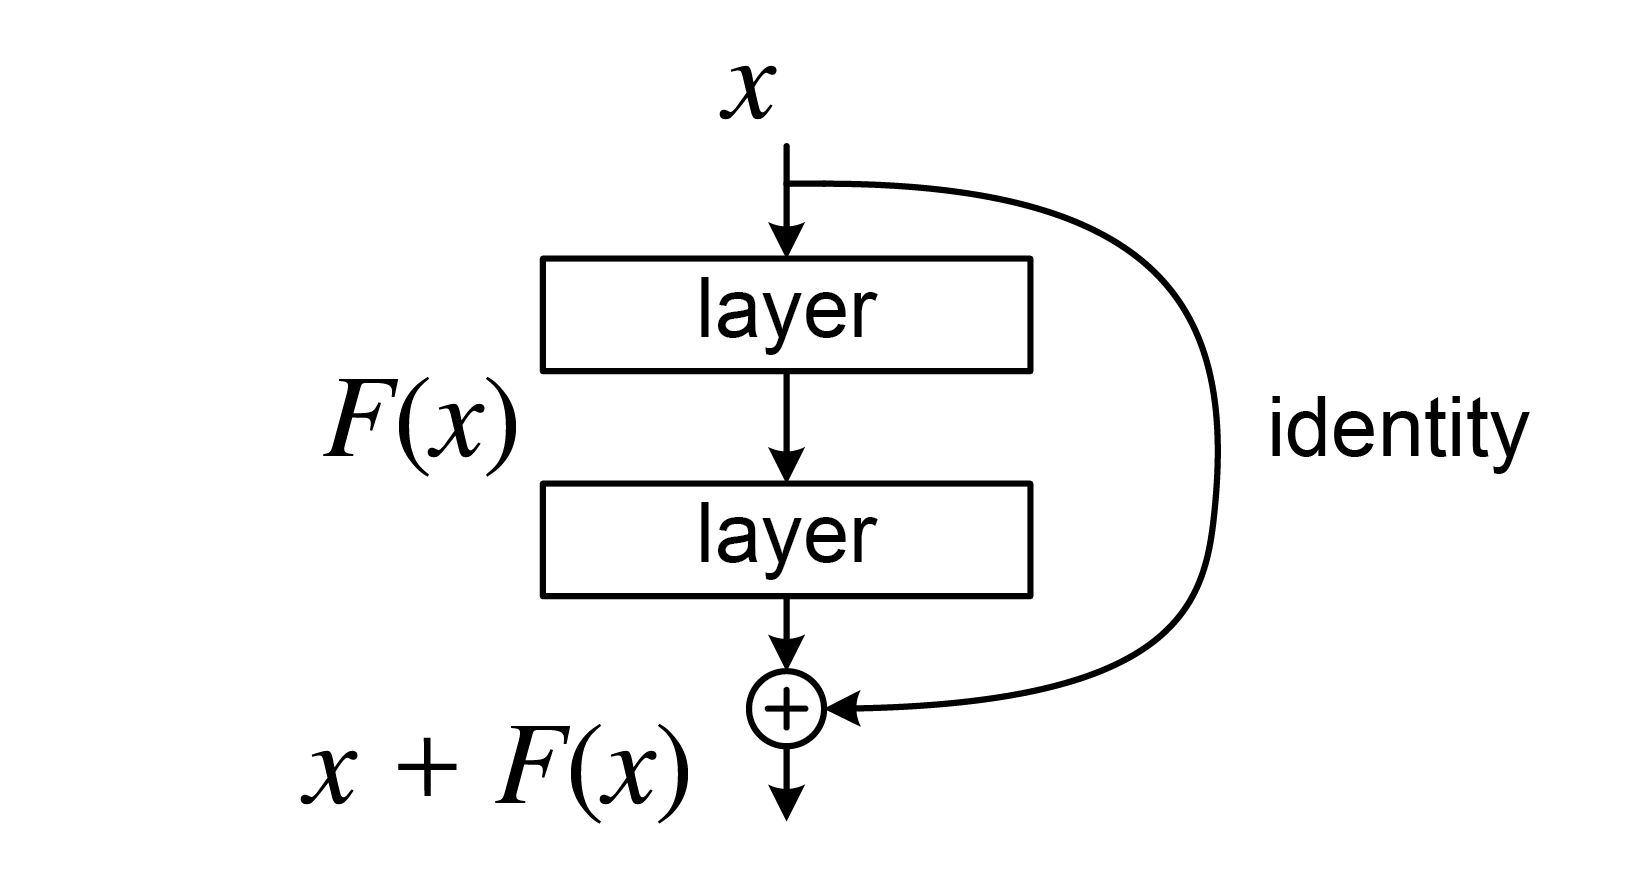
\includegraphics[width=0.7\textwidth]{img/residual_block.png}  
  \caption{Residual block \cite{residual_block_image}.}
  \label{fig:residual_block}
\end{figure}

When the convolutional layers change the spatial dimensions or number of channels, direct addition is not possible. In such cases, the shortcut connection is implemented using a $1\times1$ convolution to align the shapes of $\mathrm{x}$ and $\mathcal{F}(\mathrm{x})$ before the addition.

\subsubsection{Squeeze and excitation block}
The Squeeze-and-Excitation (SE) block was introduced in \cite{hu2018squeeze} (CVPR 2018)  the paper Squeeze-and-Excitation Networks (CVPR 2018). Its idea is to improve the representational power of CNNs by explicitly modeling interdependencies between channels.

The SE block has two main stages:

\begin{itemize}
	\item \textbf{Squeeze:} The spatial information in each channel is aggregated into a single scalar value by global average pooling. This operation reduces the spatial dimensions. For a feature map of shape $H \times W \times C$, the output of the squeeze step is a vector of length $C$.
	
	\item \textbf{Excitation:} This squeezed vector is passed through a small bottleneck feedforward neural network (typically a two-layer MLP with a ReLU activation followed by a sigmoid). The output is a set of channel-wise importance weights, one per feature channel. These weights are then used to rescale the original feature map by simple channel-wise multiplication. The network learns to emphasize important features and suppress less useful ones.
\end{itemize}

\begin{figure}[h]
  \centering
  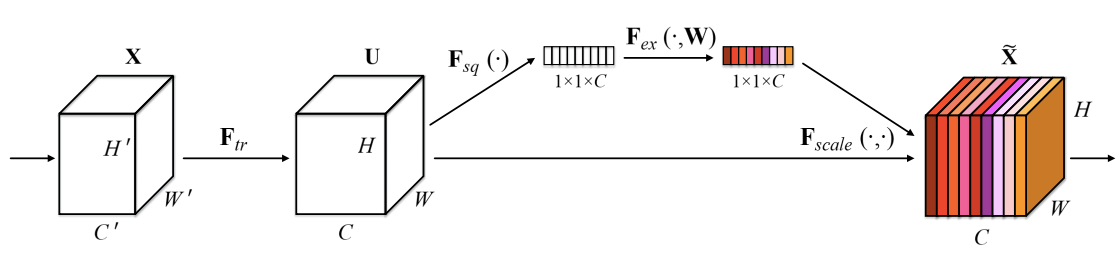
\includegraphics[width=0.9\textwidth]{img/se_scheme.png}  
  \caption{Squeeze and excitation scheme, adopted from \cite{hu2018squeeze}.}
  \label{fig:se_scheme}
\end{figure}

\subsubsection{CBAM block}
The Convolutional Block Attention Module (CBAM) enhances feature representations by sequentially applying attention mechanisms along both the channel and spatial dimensions. Unlike the Squeeze-and-Excite block, which focuses solely on channel-wise attention, CBAM extends this idea to also include spatial attention, allowing the network to emphasize what and where to attend.

For a given input feature map $\bm{F} \in \mathbb{R}^{C \times H \times W}$, CBAM applies a channel attention module followed by a spatial attention module. The channel attention module aggregates spatial information using global average and max pooling, followed by shared MLP layers, resulting in a channel attention map $M_c \in \mathbb{R}^{C \times 1 \times 1}$. The input is then refined as:

\begin{equation}
	\bm{F'} = M_c(\bm{F}) \cdot \bm{F},
\end{equation}

Next, the spatial attention module focuses on where to emphasize by applying a similar pooling and convolutional process to generate a spatial attention map $M_s \in \mathbb{R}^{1 \times H \times W}$. The final output is:

\begin{equation}
	\bm{F''} = M_s(\bm{F'}) \cdot \bm{F'},
\end{equation}

where $\cdot$ denotes element-wise multiplication.

\begin{figure}[h]
	\centering
	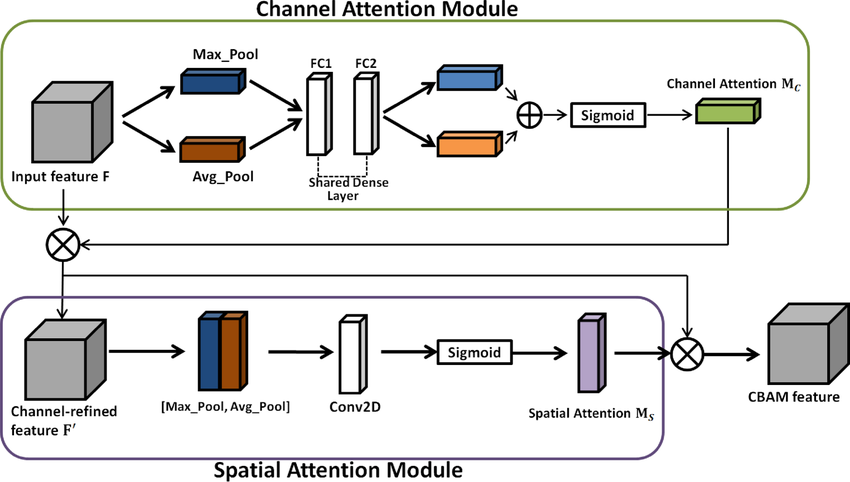
\includegraphics[width=0.9\textwidth]{img/cbam_block.png}
	\caption{CBAM block \cite{cbam_block_image}.}
	\label{fig:cbam_block}
\end{figure}

By incorporating both attention types in a lightweight and modular fashion, CBAM can be easily integrated into existing convolutional architectures to improve representational power and performance.

\subsubsection{Optimizers}

The term \emph{optimizer} defines the update rule for the model's weights during training, regardless on the concrete architecture. While the training is based on gradient decent, the choice of optimizer can significantly impact convergence and the resulting generalization. In this subsection, we briefly describe the three optimizers used in this thesis: \emph{Nesterov SGD with momentum}, \emph{RMSProp}, and \emph{AdamW}.

\paragraph{Nesterov SGD with momentum}

Standard stochastic gradient descent (SGD) can be slow to converge and sensitive to the learning rate. The \emph{momentum} technique helps accelerate convergence by smoothing updates, maintaining a velocity vector that accumulates past gradients:

\begin{equation}
    v_t = \beta v_{t-1} + \nabla_\theta \mathcal{L}(\theta),
    \label{eq:momentum_velocity_sgd}
\end{equation}

\begin{equation}
    \theta \leftarrow \theta - \alpha v_t,
    \label{eq:momentum_update_sgd}
\end{equation}

where $\beta \in [0,1)$ is the momentum coefficient.  

\emph{Nesterov momentum} \cite{sutskever2013importance} is a method that looks ahead to the estimated future position before computing the gradient:

\begin{equation}
    v_t = \beta v_{t-1} + \nabla_\theta \mathcal{L}(\theta - \alpha \beta v_{t-1}),
    \label{eq:nesterov_velocity}
\end{equation}

\begin{equation}
    \theta \leftarrow \theta - \alpha v_t.
    \label{eq:nesterov_update}
\end{equation}

This step can improve convergence, therefore we use SGD with Nesterov momentum as one of the optimizers in our experiments.

\paragraph{RMSProp}

\emph{RMSProp} was designed to address slow convergence by using adaptive learning rate. RMSProp does it by maintaining an exponentially decaying average of squared gradients:

\begin{equation}
    E[g^2]_t = \beta E[g^2]_{t-1} + (1 - \beta) (\nabla_\theta \mathcal{L}(\theta))^2,
    \label{eq:rmsprop_ema_new}
\end{equation}

\begin{equation}
    \theta \leftarrow \theta - \frac{\alpha}{\sqrt{E[g^2]_t} + \epsilon} \nabla_\theta \mathcal{L}(\theta),
    \label{eq:rmsprop_update_new}
\end{equation}

where $\beta$ is the decay rate (often set around 0.9) and $\epsilon$ is a small constant for numerical stability. By adapting learning rates individually for each parameter, RMSProp can handle noisy gradients and sharp minima effectively. We use RMSProp in selected experiments to evaluate its impact on training dynamics and generalization.

\subsubsection{Decay scheduling}
\label{subsec:decay-scheduling}

Decay scheduling changes the learning rate during training. The general idea is that as the training progresses, we want to be more conservative with the weight updates, which can be achieved by lowering the learning rate. Even though some optimizers adapt the learning rate during the training, it can still be beneficial to use scheduling. 

\paragraph{None}
The simplest approach is to keep the learning rate constant throughout the training process. However, this usually leads to suboptimal results in more complex settings.

\paragraph{Linear decay}
In linear decay, the learning rate is reduced linearly from its initial value to a predefined minimum value over the course of training. It is one of the simplest decay strategies. Suppose that $l_0$ is the initial learning rate and $T$ is the total number of steps, then the learning rate at step $t$ is:

\begin{equation} 
	\label{eq:linear-decay} 
	l_t = l_0 \left(1 - \frac{t}{T}\right). 
\end{equation}

\paragraph{Exponential decay}
Exponential decay reduces the learning rate multiplicatively at each step, resulting in a very fast decay, potentially resulting in a rapid early convergence. The formula is:

\begin{equation} 
	\label{eq:exponential-decay} 
	l_t = l_0 , \gamma^{t}, 
\end{equation}

where $\gamma \in (0,1)$ is the decay rate per step or per epoch.

\paragraph{Cosine decay}
Cosine decay schedule reduces the learning rate following a cosine function. It starts at the maximum learning rate and gradually decays to the minimum value:

\begin{equation} 
	\label{eq:cosine-decay} 
	l_t = l_{\mathrm{min}} + \frac{1}{2}(l_0 - l_{\mathrm{min}}) \left(1 + \cos\left( \pi \frac{t}{T} \right) \right)
\end{equation}

where $l_{\mathrm{min}}$ is the final learning rate. In our experiments, we use $l_0 = 0.1$ and $l_{\mathrm{min}} = \SI{1e-4}{}$ everywhere applicable.

\paragraph{Piecewise decay}
Piecewise decay divides the training process into several stages, within which the learning rate remains constant. After each stage, the learning rate is manually reduced, often by a factor of $10$. It can be seen as a crude approximation of an optimal decay schedule and is widely used in practice, especially when training dynamics are well-understood.

\paragraph{Plateau-based decay}
Plateau-based methods are similar to piecewise decay, but they monitor some metric and reduce the learning rate by some factor whenever the metric stops improving for a certain number of epochs. Our implementation follows the validation loss, and if the loss doesn't improve in the last $15$ epochs, we divide the current learning rate by a factor of $10$.

\subsection{Initialization}

Deep networks can suffer from either exploding and vanishing gradients, which naturally results in poorly performing models. The important work of \cite{glorot2010understanding} showed that this issue can be improved by proper initialization of the weights. For both dense and convolutional layers, a common strategy is to initialize weights from distributions that take into account the number of input and output units. In the mentioned paper, authors proposed so called Xavier (or Glorot) initialization. It uses a variance of $\frac{2}{n_{\text{in}} + n_{\text{out}}}$, balancing the forward and backward signal flow across layers. This initialization works reasonably well in both dense and convolutional layers when the activation function is symmetric around zero.

For networks with ReLU activations, one widely adopted initialization method is the He initialization \cite{he2015delving}, also known as Kaiming initialization. It draws weights from a zero-mean Gaussian distribution with variance $\frac{2}{n_{\text{in}}}$, where $n_{\text{in}}$ is the number of input connections to the neuron. 

For convolutional layers, these principles are applied in a spatially-aware manner, where $n_{\text{in}}$ and $n_{\text{out}}$ correspond to the number of input and output channels multiplied by the kernel size.

\subsection{Underfitting/overfitting}
A central challenge in training neural networks is ensuring that the model not only performs well on the training data but also generalizes to unseen examples. Two common failure modes are:
\begin{itemize}
    \item \textbf{Underfitting:} The model is too simple or not sufficiently trained and fails to capture the underlying patterns in the data. Both training and test performance are poor.
    \item \textbf{Overfitting:} The model is too complex or trained for too long and starts to memorize the training data, including noise. While training performance is excellent, test performance degrades.
\end{itemize}
These phenomena can be visualized by tracking the training and validation loss over time. In underfitting, both losses remain high. In overfitting, the training loss continues to drop while the validation loss increases. If the model performs well on previously unseen data, we say it \emph{generalizes} well. In our case, we don't want achieve just low test error, we want to model to generalize even further a to behave well on unlabeled data from phase transitions containing a mixture of phases.

\section{Regularization}

\emph{Regularization} is a set of techniques to prevent overfitting, \textit{(improve generalization)}, often at the cost of increasing the training error. There are many strategies to improve generalization \cite{bengio2017deep}, often at the cost of increasing the training error. In this thesis we explore following regularization strategies: constraining model parameters, modifying the objective function, altering training data, inferfering with the training process. We will describe the strategies relevant to our work in the following section.

\subsection{Parameter-norm penalties}
A common way to regularize, is to limit the capacity of a given model. This can be achieved by adding parameter-norm $\Omega(\bm{\theta})$ to the loss function $L(\bm{x} \mid \bm{\theta})$ \cite{bengio2017deep}. 

\begin{equation}
	\label{eq:loss-parameter-norm}
	\tilde{L(\bm{x} \mid \bm{\theta})} = L(\bm{x} \mid \bm{\theta}) + \lambda \Omega(\bm{\theta}),
\end{equation}
where $\lambda \geq 0$ is a hyperparameter weighting the contribution of the parameter-norm to the overall loss function.

This change means that will try to minize both the original loss function and some norm of the models parameters during the training. Noticeably $\Omega$ doesn't have to penalize all the parameters $\bm{\theta}$, in fact it is recommended to reagularize only proper weights $\bm{w}$ (leaving the biases $\bm{b}$ out) in this manner. While proper weights try to capture capture interactions between pairs of variables, biases only shifts the overall output. Large biases do not increase variability in activations and on the other hand having a large bias might be sometimes preferable. Therefore penalizing the biases in this way can cause significant and unnecessary underfitting. The most common parameter norms is the $L^2$:

\begin{equation}
 	\label{eq:l2-regularization}
 	\Omega(\bm{\theta}) = \dfrac{1}{2} ||\bm{w}||_2^2,
\end{equation} 

%and $L^1$:
%\begin{equation}
%	\label{eq:l1-regularization}
%	\Omega(\bm{\theta}) = \dfrac{1}{2} ||\bm{w}||_1.
%\end{equation} 

\subsection{Weight decay}
A weight decay is very similar to $L^2$ regularization, but is implemented little differently. Instead of changing the loss functio
n, it modifies the weight update rule during minimization. Specifically, the weights are updated as:
\begin{equation}
\bm{w} \leftarrow \bm{w} - \eta \left( \nabla_{\bm{w}} \mathcal{L} + \lambda \bm{w} \right),
\end{equation}

\subsection{Data augmentation}

The best way to improve generalization of machine learning model, is to train it on larger dataset. Getting new data is not always possible, but we can help ourselves by modifying data we already have. We can take advantage of a fact that the physical properties that define the phase of a magnetic configuration, are preserved with respect to some image tranformations. These include:
\begin{itemize}
    \item \textbf{Reflextions and $\mathbf{\ang{90}}$ rotations}: Reflexted and/or rotated configurations are entirely equivalent with respect to each other.
    \item \textbf{Rolls}: Due to periodic boundary conditions used in the Monte Carlo simulations, we can “roll” images (shift circularly) in any direction.
    \item \textbf{Global spin rotation (in-plane)}: For ferromagnetic states, we can uniformly rotate all spins, especially within the $xy$-plane, to emphasize that the essential feature is uniformity, not orientation.
\end{itemize}

We can expect that the neural networks that use these augmentations are more robust and better at generalizing across physically equivalent configurations.

Yet this is not the only benefit data augmentation brings for our usecase. We can also combine images from different classes in order to help our model recognize phase transitions. There are two common approaches for such data augmentation combining multiple classes, CutMix and MixUp. CutMix works by taking a portion of image 1 (usually rectangular segment) and pasting it onto an image 2. Resulting image will get label that is a weighted sum of original one-hot encoded labels, with weights proportional to number of pixels contributed by each image. MixUp works again by taking two images, generating random number $\alpha \in (0, 1)$ and adding pixels of these images weighted by $\alpha$ (resp. $1 - \alpha$). Label is then created in same manner.

\begin{figure}[ht]
  \centering
  \begin{subfigure}[b]{0.22\textwidth}
    \centering
    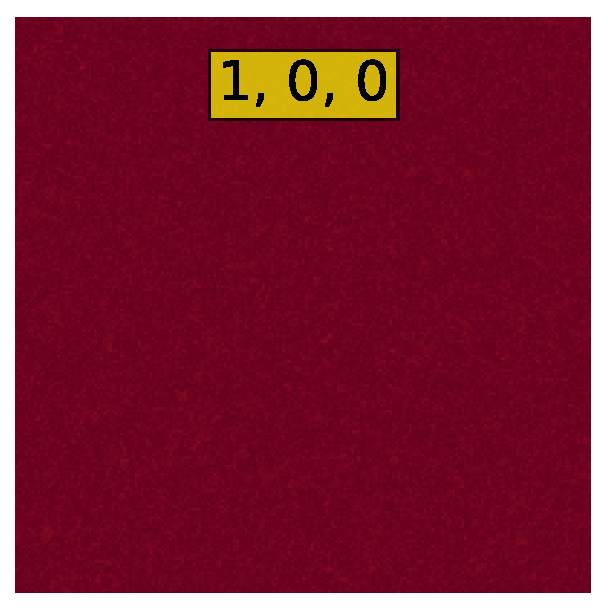
\includegraphics[width=\textwidth]{img/augment_fe_1.pdf}
    \caption{Ferromagnet}
    \label{fig:aug_fe_1}
  \end{subfigure}
	\centering
  \begin{subfigure}[b]{0.22\textwidth}
    \centering
    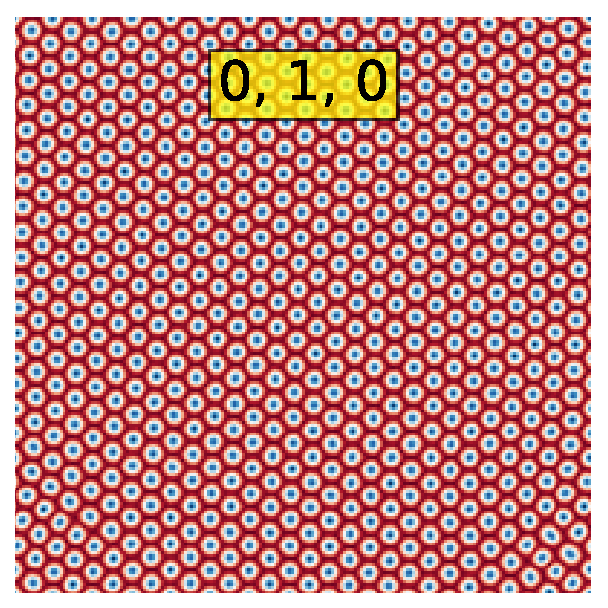
\includegraphics[width=\textwidth]{img/augment_fe_2.pdf}
    \caption{Skyrmion latice}
    \label{fig:aug_fe_2}
  \end{subfigure}
  \centering
  \begin{subfigure}[b]{0.22\textwidth}
    \centering
    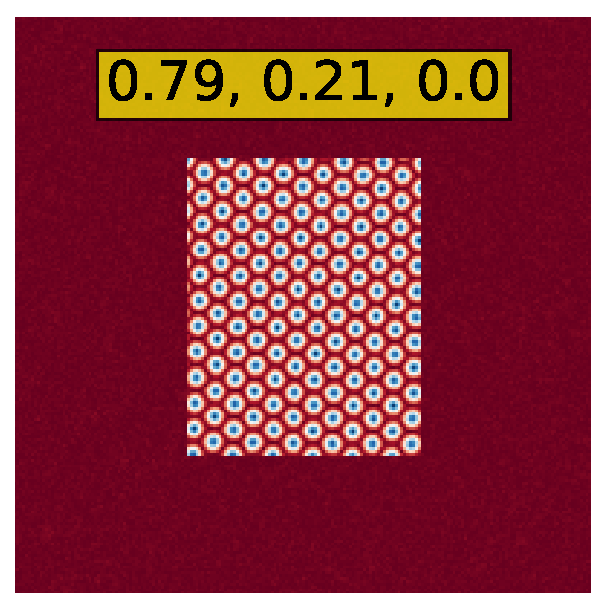
\includegraphics[width=\textwidth]{img/augment_fe_3.pdf}
    \caption{CutMix}
    \label{fig:aug_fe_3}
  \end{subfigure}
  \centering
  \begin{subfigure}[b]{0.22\textwidth}
    \centering
    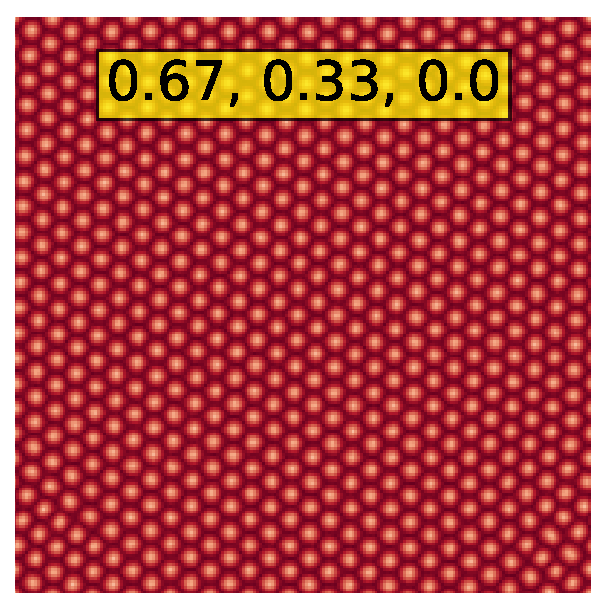
\includegraphics[width=\textwidth]{img/augment_fe_4.pdf}
    \caption{MixUp}
    \label{fig:aug_fe_4}
  \end{subfigure}
  \caption{Augmentation between ferromagnet and skyrmion phases.}
  \label{fig:aug_fe}
\end{figure}

\begin{figure}[ht]
  \centering
  \begin{subfigure}[b]{0.22\textwidth}
    \centering
    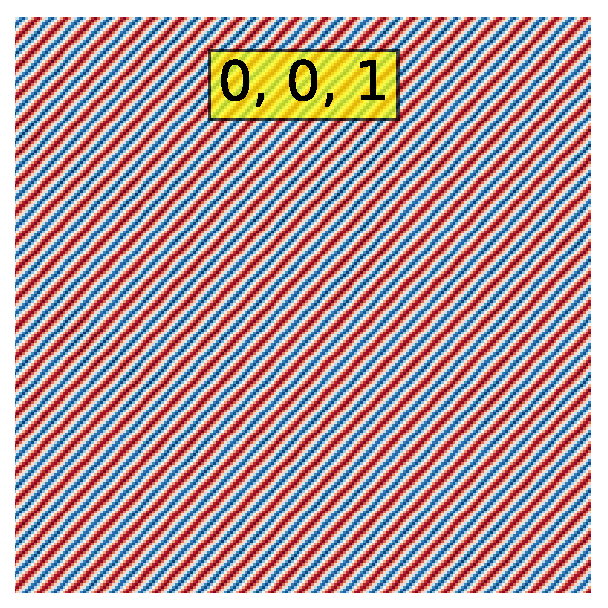
\includegraphics[width=\textwidth]{img/augment_sp_1.pdf}
    \caption{Ferromagnet}
    \label{fig:aug_sp_1}
  \end{subfigure}
	\centering
  \begin{subfigure}[b]{0.22\textwidth}
    \centering
    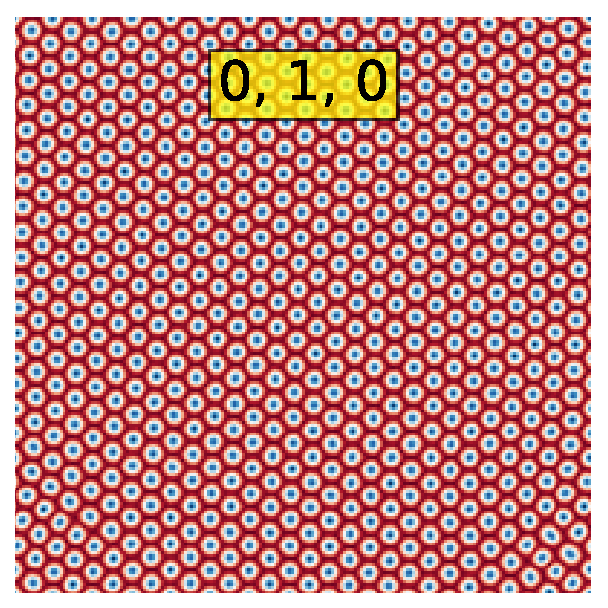
\includegraphics[width=\textwidth]{img/augment_sp_2.pdf}
    \caption{Skyrmion latice}
    \label{fig:aug_sp_2}
  \end{subfigure}
  \centering
  \begin{subfigure}[b]{0.22\textwidth}
    \centering
    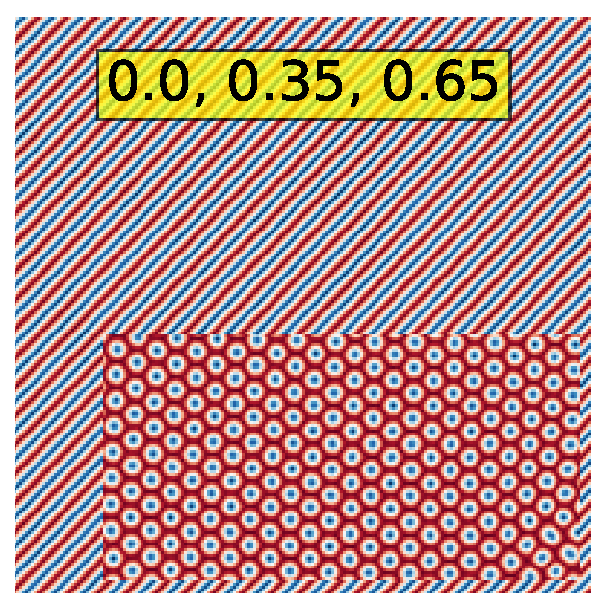
\includegraphics[width=\textwidth]{img/augment_sp_3.pdf}
    \caption{CutMix}
    \label{fig:aug_sp_3}
  \end{subfigure}
  \centering
  \begin{subfigure}[b]{0.22\textwidth}
    \centering
    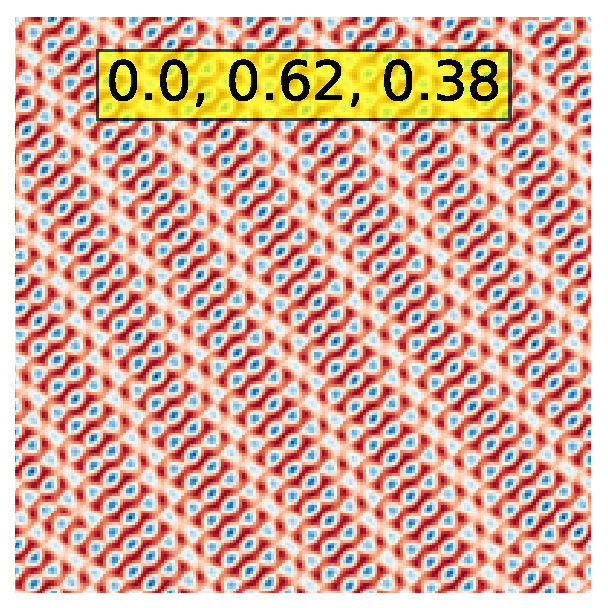
\includegraphics[width=\textwidth]{img/augment_sp_4.pdf}
    \caption{MixUp}
    \label{fig:aug_sp_4}
  \end{subfigure}
  \caption{Augmentation between ferromagnet and skyrmion phases.}
  \label{fig:aug_sp}
\end{figure}

\subsection{Dropout}

\emph{Dropout} \cite{srivastava2014dropout} is a regularization technique for preventing overfitting by randomly switching of activations during training. For dense networks, individual neurons are independently set to zero with probability $p$, typically $p \in [0, 0.5]$. To balance the loss of the overall signal magnitude during training, we usually scale the remaining activations by a factor $\nicefrac{1}{p}$. Dropout is then disabled during the inference.

Dropout can be applied also in convolutional layers with some modification. Standard dropout would remove individual pixels, which may not be effective due to spatial correlations. Therefore, it is common to use \emph{SpatialDropout} \cite{tompson2015efficient}, which drops entire feature maps (channels) or \emph{DropBlock} which drops entire rectangular block of feature. Implementation of DropBlock doesn't make sense for our usecase, sinse we try to evaluate how much of each phase is present in the given image. Which leaves us with the spatial dropout for convolutional layes as only viable option.

\subsection{Monte Carlo Dropout}

Monte Carlo dropout is in it's idea closely connected to the \emph{model ensembling}. Model ensembling is a regularization technique that combines multiple models. The intuition is that individual models make different errors, and averaging their predictions reduces the variance and improves the robustness. The drawback of model ensembling is the computational cost. It is costly to train many models, just to average their predictions. However, we can approximate the model ensemble by using the \emph{Monte-Carlo (MC) dropout} \cite{gal2016dropout}. Monte Carlo dropout extends the idea of dropout to the inference. Instead of disabling dropout during the inference, we can keep it active and perform multiple forward passes. Each forward pass samples a different subnetwork from the full model, effectively creating an ensemble.

\subsection{Early Stopping}

\emph{Early stopping} \cite{prechelt2002early} is a regularization technique that directly interfere with the training process. It requires additional \emph{validation} dataset, that is not used for updating weights. We use it to monitor a  validation loss during training, and instead of training for a fixed number of steps, we stop as soon as the validation loss stops improving (for certain number of epochs, in our case $40$). This stops the model from overtraining, improving the generalization. After early stopping, we restore the model's weights from the epoch with minimal validation loss.